\section{Methodology}

The design of our model is based on conversational features such as dialog structure (the order and boundaries of the utterances) and the attribution of each utterance to its corresponding speaker. The model architecture, inspired by \citet{li2020hierarchical}, is shown in Figure \ref{pipeline}. 
PRIDE hierarchically creates word and utterance representations, which are then combined with representations of personal attributes and interpersonal dimensions (Table \ref{dimensions}) to create a representation of the full conversation history.
Given this representation of the conversation, a multi-label classification layer predicts one or more of the relationship labels, listed in Table \ref{perclass}.
The model is trained with supervision on the relationship labels.
In the following subsections we describe the model's components in more detail.

\begin{figure}[t!]
\centering
\begin{adjustbox}{width=0.6\textwidth}
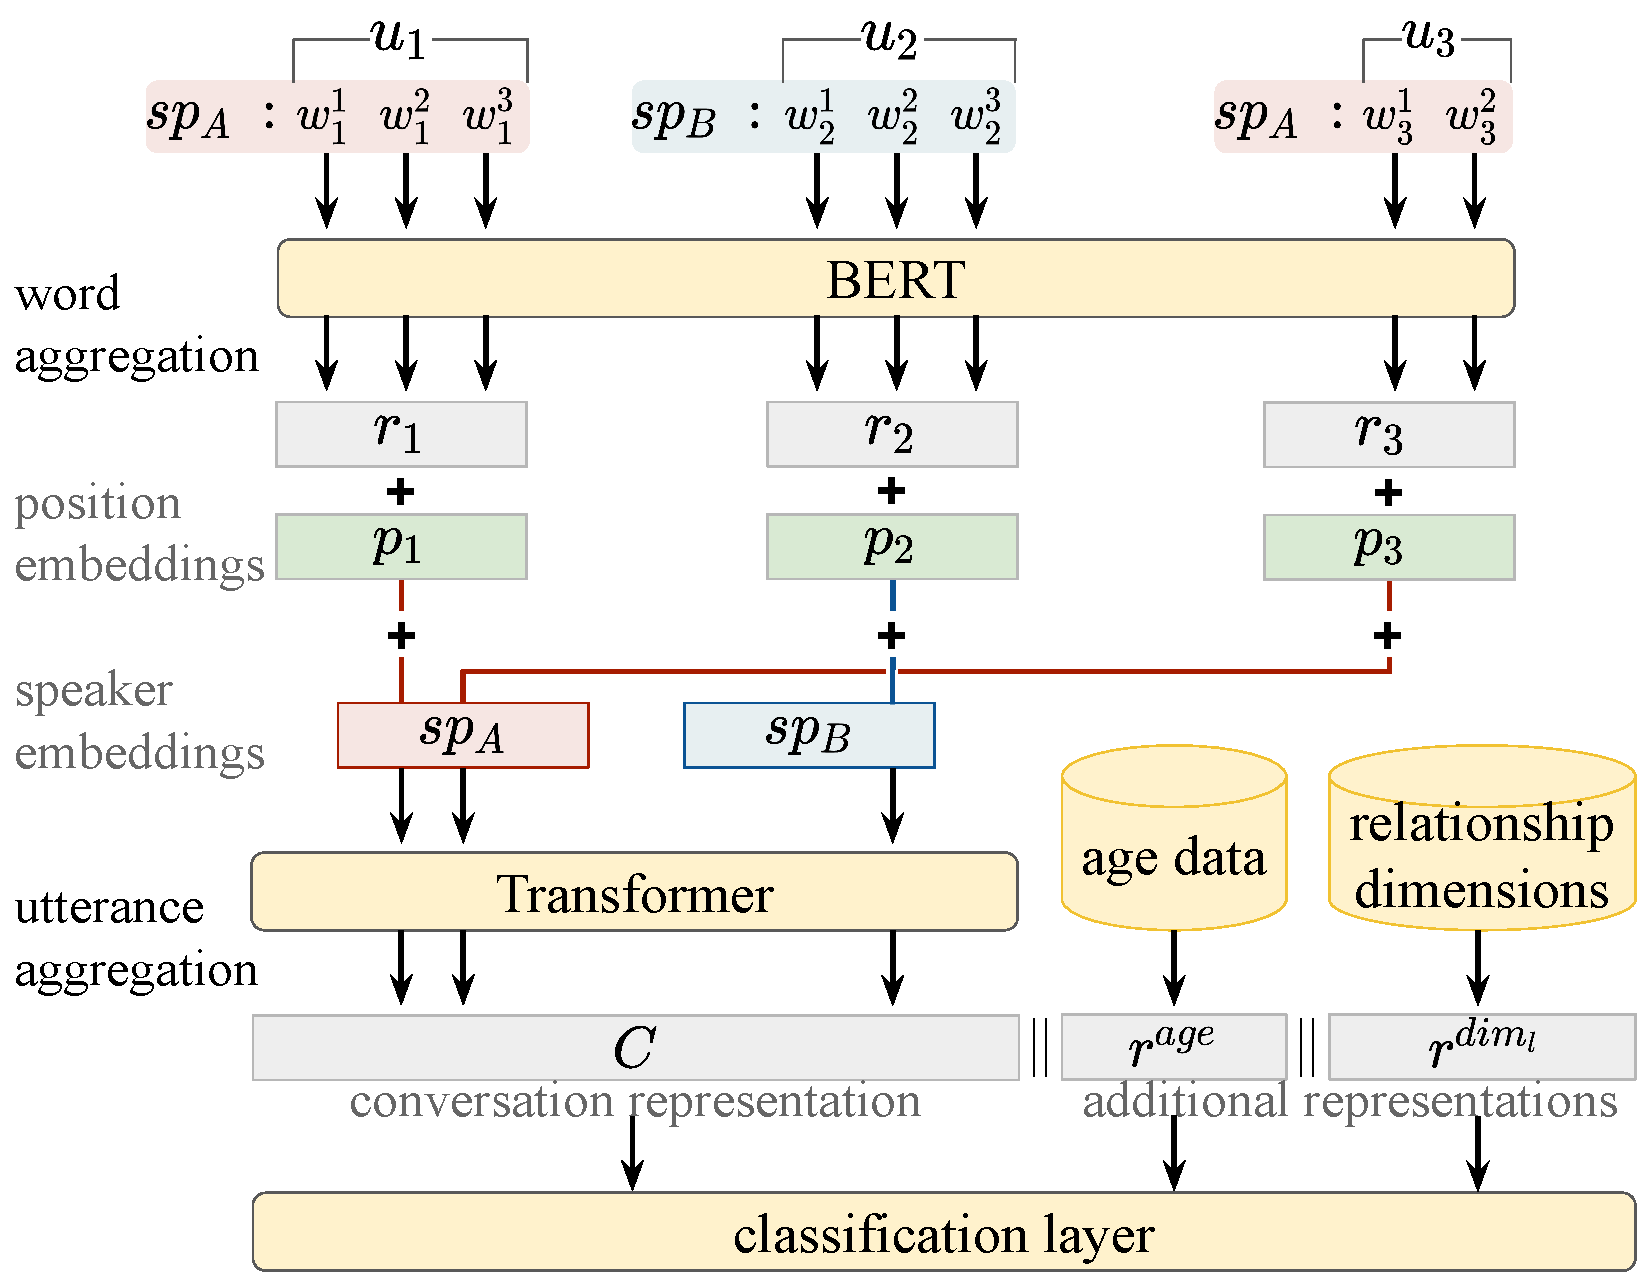
\includegraphics{imgs/PRIDE_scheme_3}
\end{adjustbox}
\caption{PRIDE model}
\label{pipeline}
\end{figure}

\subsection{Contextual word representations}

The input for a pair of speakers ($sp_A$, $sp_B$) is $N$ utterances $u_1, ... u_N$, where $i$-th utterance consists of words $w_i^1, ... w_i^{n_i}$. 
In the first step, the word representations $r_i^j$ are created with a function $f^{word}(w_1^1,..,w_1^{n_1},...,w_N^{n_N})=r_i^j$, which takes as input the concatenation of all utterances and produces the representations for each word. We chose BERT \cite{devlin2019bert} to create word representations, because this model efficiently captures contextual information.

Considering that the maximal input length of BERT is 512 tokens, we split the input sequence of utterances into chunks and run BERT several times. Each chunk in the split has the maximal possible length that fits into one run without breaking individual utterances. We find this splitting strategy more effective than running BERT on single utterances \cite{chen2020mpdd} or short sequences which don't fully utilize max 512 limit \cite{jia2020ddrel}. In our method more conversational context is provided to create word representations. Also, simply truncating input to 512 tokens \cite{lu2020improving} might cause a loss of important cues. 

As information about the current speaker we use BERT's segment embeddings, so that the A-segment corresponds to tokens from $sp_A$ and the B-segment to $sp_B$.
Furthermore, we encode the information about the utterance boundaries by prepending special tokens before each utterance: $[\textrm{s1}]$ for the utterances of speaker A and $[\textrm{s2}]$ for speaker B. 

\subsection{Utterance representations}

Next, word representations $r_i^j$ are aggregated within each utterance to create utterance representations $r_i$ with the aggregation function $a^{word}(r_i^1,...r_i^{n_i})=r_i$. The aggregation is performed on the utterances from all runs of BERT and outputs $r_1, ... r_N$ as the representations of utterances.
In our hyperparameter search we tried instantiating $a^{word}$ with \textit{max}, \textit{average} and \textit{self-attention weighted average} functions.

Some of $\hat{r_i}$ are been produced by separate runs of BERT due to its input length limitation. Therefore we create enriched utterance representations in the unified context from all BERT runs with the function $f^{utt}(\hat{r}_1,...,\hat{r}_n) = \tilde{r_i}$. We instantiate $f^{utt}$ with a Transformer encoder, which allows us to input long sequences of utterances. 
Before computing enriched representations, we sum the utterance representations $r_i$ with sinusoidal positional encoding $p_i$ and speaker embeddings $sp_i$, yielding $\hat{r_i} = r_i + p_i + sp_i$. The speaker embeddings are randomly initialized and learned during model training. Positional encoding is performed following \citet{vaswani2017attention}. 

\subsection{Classification layer}

Finally, the enriched utterance representations $\tilde{r_i}$ are aggregated with the function ${a^{utt}(\tilde{r_1},...\tilde{r_n})=C}$. 
$a^{utt}$ is instantiated with the same aggregation functions as $a^{word}$. For the case with $[\textrm{CLS}]$ representation we prepend a trainable embedding to the sequence.

We incorporate additional information relevant to the relationship prediction by concatenating embeddings of personal attributes and interpersonal dimensions with the conversation representation $C$: $\tilde{C} = C|r^{age}|r_{dim_l}$, which are described in the following subsections.
A fully connected layer takes the resulting concatenated representation $\tilde{C}$ as input and produces probability scores for each of $L$ relationship labels. Since some relationships are not symmetric (e.g., \emph{parent/child}) the labels represent directed relationships from $sp_A$ to $sp_B$.


\subsection{Incorporating personal attributes}

Additional personal information about the speakers from a personal knowledge base, such as their age or occupation, could improve relationship prediction.
We incorporate \textit{age} information into the model, since some relationships in our dataset can commonly be characterized by age differences between the speakers. For instance, children are usually much younger than their parents (and a parent can never be younger than a child). Similarly, employees are generally younger than their bosses (but the magnitude of their age difference is less than in parent/child pairs). We incorporate only age difference for two reasons: (i) other labeled personal attributes are very scarce and difficult to obtain, and (ii) other attributes, such as gender, are not nearly as informative as speakers' age difference. Nevertheless, the architecture of PRIDE can easily include any number of additional attributes (e.g., profession, marital status, etc.).

To incorporate age information into PRIDE, we introduce a representation for the age difference of speakers. We calculate $(age_A - age_B)$ and assign the resulting difference into an age difference bin.
We learn an $m$-dimensional embedding $r^{age}$  for each bin, where $m$ is a hyperparameter optimized in the grid search.

\subsection{Incorporating interpersonal dimensions}

As discussed in Section \ref{background}, interpersonal relationships have fine-grained characteristics, called \textit{dimensions} \cite{wish1976perceived}. For instance, a \textit{boss/employee} relationship is hierarchical, while \textit{colleague} is an equal one. Similarly, \textit{spouse} is an intimate relationship, in contrast with \textit{colleague}.

Given a hint of the applicable dimensions, a model can better predict the underlying relationship (e.g., a \textit{non-intimate}, \textit{task oriented} and \textit{hierarchical} relationship is most likely a \textit{boss/employee} relationship). Based on \citet{rashid2018characterizing}, we distinguish 11 interesting interpersonal dimensions listed in Table \ref{dimensions}. 

Using the data provided by \citet{rashid2018characterizing} we train a separate BERT classifier on the utterance level for each dimension $dim_l$, where index $l$ ranges over the 11 interpersonal dimensions we used.
We obtain a $K$-dimensional CLS representation from the trained classifier for each utterance, thus producing a $K$-dimensional representations $r^{dim_l}_i$ for the $i$-th input utterance.
To incorporate these representations into our model, we obtain a single representation $dim_l$ at the conversation level by performing max pooling over all utterance representations for a given speaker pair.

